\documentclass[journal,12pt,twocolumn]{IEEEtran}

\usepackage{setspace}
\usepackage{gensymb}

\singlespacing


\usepackage[cmex10]{amsmath}

\usepackage{amsthm}

\usepackage{mathrsfs}
\usepackage{txfonts}
\usepackage{stfloats}
\usepackage{bm}
\usepackage{cite}
\usepackage{cases}
\usepackage{subfig}

\usepackage{longtable}
\usepackage{multirow}

\usepackage{enumitem}
\usepackage{mathtools}
\usepackage{steinmetz}
\usepackage{tikz}
\usepackage{circuitikz}
\usepackage{verbatim}
\usepackage{tfrupee}
\usepackage[breaklinks=true]{hyperref}
\usepackage{graphicx}
\usepackage{tkz-euclide}
\usepackage{float}

\usetikzlibrary{calc,math}
\usepackage{listings}
    \usepackage{color}                                            %%
    \usepackage{array}                                            %%
    \usepackage{longtable}                                        %%
    \usepackage{calc}                                             %%
    \usepackage{multirow}                                         %%
    \usepackage{hhline}                                           %%
    \usepackage{ifthen}                                           %%
    \usepackage{lscape}     
\usepackage{multicol}
\usepackage{chngcntr}

\DeclareMathOperator*{\Res}{Res}

\renewcommand\thesection{\arabic{section}}
\renewcommand\thesubsection{\thesection.\arabic{subsection}}
\renewcommand\thesubsubsection{\thesubsection.\arabic{subsubsection}}

\renewcommand\thesectiondis{\arabic{section}}
\renewcommand\thesubsectiondis{\thesectiondis.\arabic{subsection}}
\renewcommand\thesubsubsectiondis{\thesubsectiondis.\arabic{subsubsection}}


\hyphenation{op-tical net-works semi-conduc-tor}
\def\inputGnumericTable{}                                 %%

\lstset{
%language=C,
frame=single, 
breaklines=true,
columns=fullflexible
}
\begin{document}
\newtheorem{theorem}{Theorem}[section]
\newtheorem{problem}{Problem}
\newtheorem{proposition}{Proposition}[section]
\newtheorem{lemma}{Lemma}[section]
\newtheorem{corollary}[theorem]{Corollary}
\newtheorem{example}{Example}[section]
\newtheorem{definition}[problem]{Definition}

\newcommand{\BEQA}{\begin{eqnarray}}
\newcommand{\EEQA}{\end{eqnarray}}
\newcommand{\define}{\stackrel{\triangle}{=}}
\bibliographystyle{IEEEtran}
\providecommand{\mbf}{\mathbf}
\providecommand{\pr}[1]{\ensuremath{\Pr\left(#1\right)}}
\providecommand{\qfunc}[1]{\ensuremath{Q\left(#1\right)}}
\providecommand{\sbrak}[1]{\ensuremath{{}\left[#1\right]}}
\providecommand{\lsbrak}[1]{\ensuremath{{}\left[#1\right.}}
\providecommand{\rsbrak}[1]{\ensuremath{{}\left.#1\right]}}
\providecommand{\brak}[1]{\ensuremath{\left(#1\right)}}
\providecommand{\lbrak}[1]{\ensuremath{\left(#1\right.}}
\providecommand{\rbrak}[1]{\ensuremath{\left.#1\right)}}
\providecommand{\cbrak}[1]{\ensuremath{\left\{#1\right\}}}
\providecommand{\lcbrak}[1]{\ensuremath{\left\{#1\right.}}
\providecommand{\rcbrak}[1]{\ensuremath{\left.#1\right\}}}
\theoremstyle{remark}
\newtheorem{rem}{Remark}
\newcommand{\sgn}{\mathop{\mathrm{sgn}}}
\providecommand{\abs}[1]{\left\vert#1\right\vert}
\providecommand{\res}[1]{\Res\displaylimits_{#1}} 
\providecommand{\norm}[1]{\left\lVert#1\right\rVert}
%\providecommand{\norm}[1]{\lVert#1\rVert}
\providecommand{\mtx}[1]{\mathbf{#1}}
\providecommand{\mean}[1]{E\left[ #1 \right]}
\providecommand{\fourier}{\overset{\mathcal{F}}{ \rightleftharpoons}}
%\providecommand{\hilbert}{\overset{\mathcal{H}}{ \rightleftharpoons}}
\providecommand{\system}{\overset{\mathcal{H}}{ \longleftrightarrow}}
	%\newcommand{\solution}[2]{\textbf{Solution:}{#1}}
\newcommand{\solution}{\noindent \textbf{Solution: }}
\newcommand{\cosec}{\,\text{cosec}\,}
\providecommand{\dec}[2]{\ensuremath{\overset{#1}{\underset{#2}{\gtrless}}}}
\newcommand{\myvec}[1]{\ensuremath{\begin{pmatrix}#1\end{pmatrix}}}
\newcommand{\mydet}[1]{\ensuremath{\begin{vmatrix}#1\end{vmatrix}}}
\numberwithin{equation}{subsection}
\makeatletter
\@addtoreset{figure}{problem}
\makeatother
\let\StandardTheFigure\thefigure
\let\vec\mathbf
\renewcommand{\thefigure}{\theproblem}
\def\putbox#1#2#3{\makebox[0in][l]{\makebox[#1][l]{}\raisebox{\baselineskip}[0in][0in]{\raisebox{#2}[0in][0in]{#3}}}}
     \def\rightbox#1{\makebox[0in][r]{#1}}
     \def\centbox#1{\makebox[0in]{#1}}
     \def\topbox#1{\raisebox{-\baselineskip}[0in][0in]{#1}}
     \def\midbox#1{\raisebox{-0.5\baselineskip}[0in][0in]{#1}}
\vspace{3cm}
\title{ASSIGNMENT 4}
\author{B.ANUSHA}
\maketitle
\newpage
\bigskip
\renewcommand{\thefigure}{\theenumi}
\renewcommand{\thetable}{\theenumi}
Download all python codes from 
\begin{lstlisting}
https://github.com/BOJJAVOYINAANUSHA/ASSIGNMENT4/tree/main/ASSIGNMENT4/assignment.py
\end{lstlisting}
%
Latex-tikz codes from 
%
\begin{lstlisting}
https://github.com/BOJJAVOYINAANUSHA/ASSIGNMENT4/tree/main/ASSIGNMENT4/ASSIGNMENT.tex
\end{lstlisting}
%
\section{Question No 2.45}
Find the equation of the normal to the curve $x^2 = 4y$ which passes through the point $\myvec{1\\2}$.
\section{SOLUTION} 
Given curve,
\begin{align}
x^2=4y\\
\implies x^2-4y =0 \label{2.0.2}
\end{align}
Comparing with the standard equation :
\begin{align}
\vec{x}^T\vec{V}\vec{x}+2\vec{u}^T\vec{x}+f=0\\
\vec{V}=\myvec{1 & 0 \\ 0 & 0},\vec{u}=\myvec{0 \\ -2 }, \vec{f} = 0 
\end{align}
$\because$
\begin{align}
 \abs{\vec{V}} &= 0
\end{align}
$\therefore$ the given curve \eqref{2.0.2} represents a parabola .
we can find the eigen values corresponding to the $\vec{V}$,
\begin{align}
\abs{\vec{V} - \lambda\vec{I}} = \mydet{1-\lambda & 0 \\ 0 & -\lambda} &= 0
\\
\implies (1- \lambda)(-\lambda) &= 0
\end{align}
$\therefore$ Eigen values are 
\begin{align}
\lambda_1 = 0 , \lambda_2 = 1
\end{align}
Calculating the eigen vectors corresponding to $\lambda_1 = 0 , \lambda_2 = 1$ respectively.
\begin{align}
\vec{V}\vec{x} &= \lambda\vec{x}
\\
\myvec{1 & 0 \\ 0 & 0}\vec{x} &=0 \implies \vec{p_1} = \myvec{0 \\ 1}
\\
\myvec{0 & 0 \\ 0 & -1}\vec{x} &=0 \implies \vec{p_2} = \myvec{1 \\ 0}
\end{align}
 By eigen decomposition on $\vec{V}$,
\begin{align}
\vec{V}=\vec{P}\vec{D}\vec{P}^T
\end{align}
Where,
\begin{align}
\vec{P} &= \myvec{\vec{p_1} & \vec{p_2}} = \myvec{0 & 1 \\ 1 & 0}
\\
\vec{D} &= \myvec{\lambda_1 & 0 \\ 0 & \lambda_2} =\myvec{0 & 0 \\ 0 & 1} 
\end{align}
To find the vertex of the parabola ,
\begin{align} \myvec{\vec{u}+\kappa\vec{p_1^T}\\\vec{V} }\vec{C} &= \myvec{\vec{-f}\\\kappa \vec{p_1} -\vec{u}}
\\
\text{where, }  \kappa = \vec{u^T}\vec{p_1} = -2
\\
\implies\myvec{0 & -4\\1 & 0 \\0 & 0} \vec{C}&= \myvec{0\\0\\0} \label{eq:b}
\end{align}
from the above it can be observed that,
\begin{align}    
   \vec{C} &= \myvec{0 \\ 0}
\end{align}
Now to evalute the direction vector m,
\begin{align}
\vec{m}^T(\vec{V}\vec{q} + \vec{u}) &=0
\\
\vec{m}^T\brak{\myvec{1 & 0 \\ 0 & 0}\myvec{1 \\ 2} + \myvec{0 \\ -2}} &=0
\\
\vec{m}^T\myvec{1 \\ -2} &=0
\\
\vec{m} = \myvec{-2 \\ -1}
\end{align}
Now to obtain the equation of normal using,
\begin{align}
\vec{m}^T(\vec{x} - \vec{q}) &=0 
\\
\myvec{-2 & -1}\brak{\vec{x}-\myvec{1 \\ 2}} &= 0
\\
\myvec{-2 & -1}\vec{x}+ 4 &= 0 
\end{align}
\begin{itemize}
\item Plot of Normal to the given curve -
\end{itemize}
\numberwithin{figure}{section}
\begin{figure}[ht]
    \centering
    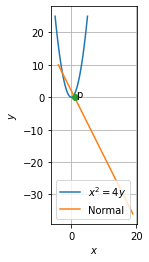
\includegraphics[width=\columnwidth]{PARABOLA.png}
    \caption{Normal to Parabola.}
    \label{fig:Normal to parabola.}
\end{figure}    
\end{document}
